\documentclass[border=12pt]{standalone}
\def\pgfsysdriver{pgfsys-dvisvgm.def}
\usepackage[dvisvgm]{xcolor}
\usepackage{xeCJK}
\setCJKmainfont{HaranoAjiGothic-Regular.otf}[BoldFont=HaranoAjiGothic-Bold.otf]
\setCJKsansfont{HaranoAjiGothic-Regular.otf}[BoldFont=HaranoAjiGothic-Bold.otf]
\usepackage{amsmath,amssymb,tikz,lmodern}
\usetikzlibrary{arrows.meta,positioning,calc}
\renewcommand{\familydefault}{\sfdefault}
\definecolor{ink}{HTML}{25322F}
\definecolor{green}{HTML}{246657}
\definecolor{tint}{HTML}{EEF4F0}
\definecolor{soft}{HTML}{C6D2CC}
\definecolor{muted}{HTML}{52615B}
\newif\ifJapanese
\newcommand{\Tx}[2]{\ifJapanese #1\else #2\fi}
\newcommand{\heading}[3]{{\color{green}\bfseries #1\quad\Tx{#2}{#3}}\\[5pt]}
\newcommand{\Var}{\operatorname{Var}}
\newcommand{\Frac}{\operatorname{Frac}}
\newcommand{\C}{\mathbb C}
\newcommand{\refurl}[2]{\special{dvisvgm:raw <a xlink:href="#1" target="_blank" rel="noopener noreferrer">}{\setlength{\fboxsep}{0pt}\colorbox{white}{\color{green}\underline{\strut #2}}}\special{dvisvgm:raw </a>}}
\newcommand{\R}[2]{\refurl{\csname source#1\endcsname}{#2}}
\tikzset{
 card/.style={draw=soft,fill=white,rounded corners=2pt,align=left,text=ink,font=\fontsize{10.5}{14}\selectfont,inner xsep=12pt,inner ysep=11pt,text width=14.4cm},
 result/.style={card,draw=green,fill=tint,line width=.9pt},
 reason/.style={align=left,text=muted,font=\fontsize{9}{12}\selectfont,inner sep=0pt,text width=12.7cm},
 edge/.style={-{Stealth[length=2.4mm]},draw=green,line width=1pt}
}
\newcommand{\flow}[3]{
 \coordinate (#2-from) at ($(#1.south)+(-6.9,0)$);
 \coordinate (#2-to) at ($(#2.north)+(-6.9,0)$);
 \draw[edge] (#2-from)--(#2-to);
 \node[reason,anchor=west] at ($(#2-from)!.5!(#2-to)+(.55,0)$) {#3};
}

\Japanesefalse
\expandafter\def\csname sourceWV\endcsname{https://github.com/openai/math/blob/fd4aeeb2ee4fc729c18d98444fed42fd0529eeeb/preprints/Logarithmic-Kodaira-dimension-and-whole-fiber-variation-September-26-2026/paper.pdf}
\expandafter\def\csname sourceOI\endcsname{https://github.com/openai/math/blob/fd4aeeb2ee4fc729c18d98444fed42fd0529eeeb/preprints/Orbifold-and-logarithmic-Iitaka-subadditivity-September-26-2026/paper.pdf}
\expandafter\def\csname sourcePH\endcsname{https://github.com/openai/math/blob/fd4aeeb2ee4fc729c18d98444fed42fd0529eeeb/preprints/Projective-Hodge-lines-and-ordinary-Iitaka-subadditivity-September-27-2026/paper.pdf}
\expandafter\def\csname sourceRA\endcsname{https://github.com/openai/math/blob/fd4aeeb2ee4fc729c18d98444fed42fd0529eeeb/preprints/The-reverse-logarithmic-Kodaira-inequality-and-additivity-September-26-2026/paper.pdf}
\expandafter\def\csname sourceLA\endcsname{https://github.com/openai/math/blob/adc7f1241b42e322a6451854ab7e4b4c146bf78a/preprints/Log-abundance-in-characteristic-zero-September-24-2026/paper.pdf}
\expandafter\def\csname sourceFuj\endcsname{https://www.math.kyoto-u.ac.jp/~fujino/weak-posi11.pdf}
\expandafter\def\csname sourceDel\endcsname{https://www.numdam.org/item/PMIHES_1971__40__5_0.pdf}
\expandafter\def\csname sourceDHP\endcsname{https://arxiv.org/pdf/1012.0493v2}
\expandafter\def\csname sourcePT\endcsname{https://arxiv.org/pdf/1409.5504v1}
\expandafter\def\csname sourceBCHM\endcsname{https://arxiv.org/pdf/math/0610203v2}
\expandafter\def\csname sourceKP\endcsname{https://sites.math.washington.edu/~kovacs/2013/papers/Kovacs_Patakfalvi__Projectivity.pdf}
\expandafter\def\csname sourceHan\endcsname{https://doi.org/10.1007/BF01394338}
\expandafter\def\csname sourceSGA1\endcsname{https://arxiv.org/abs/math/0206203v2}
\expandafter\def\csname sourceLan\endcsname{https://arxiv.org/pdf/2005.09690v3}
\expandafter\def\csname sourceBDPP\endcsname{https://arxiv.org/pdf/math/0405285v1}
\expandafter\def\csname sourceTaj\endcsname{https://arxiv.org/pdf/2005.01025v4}
\begin{document}
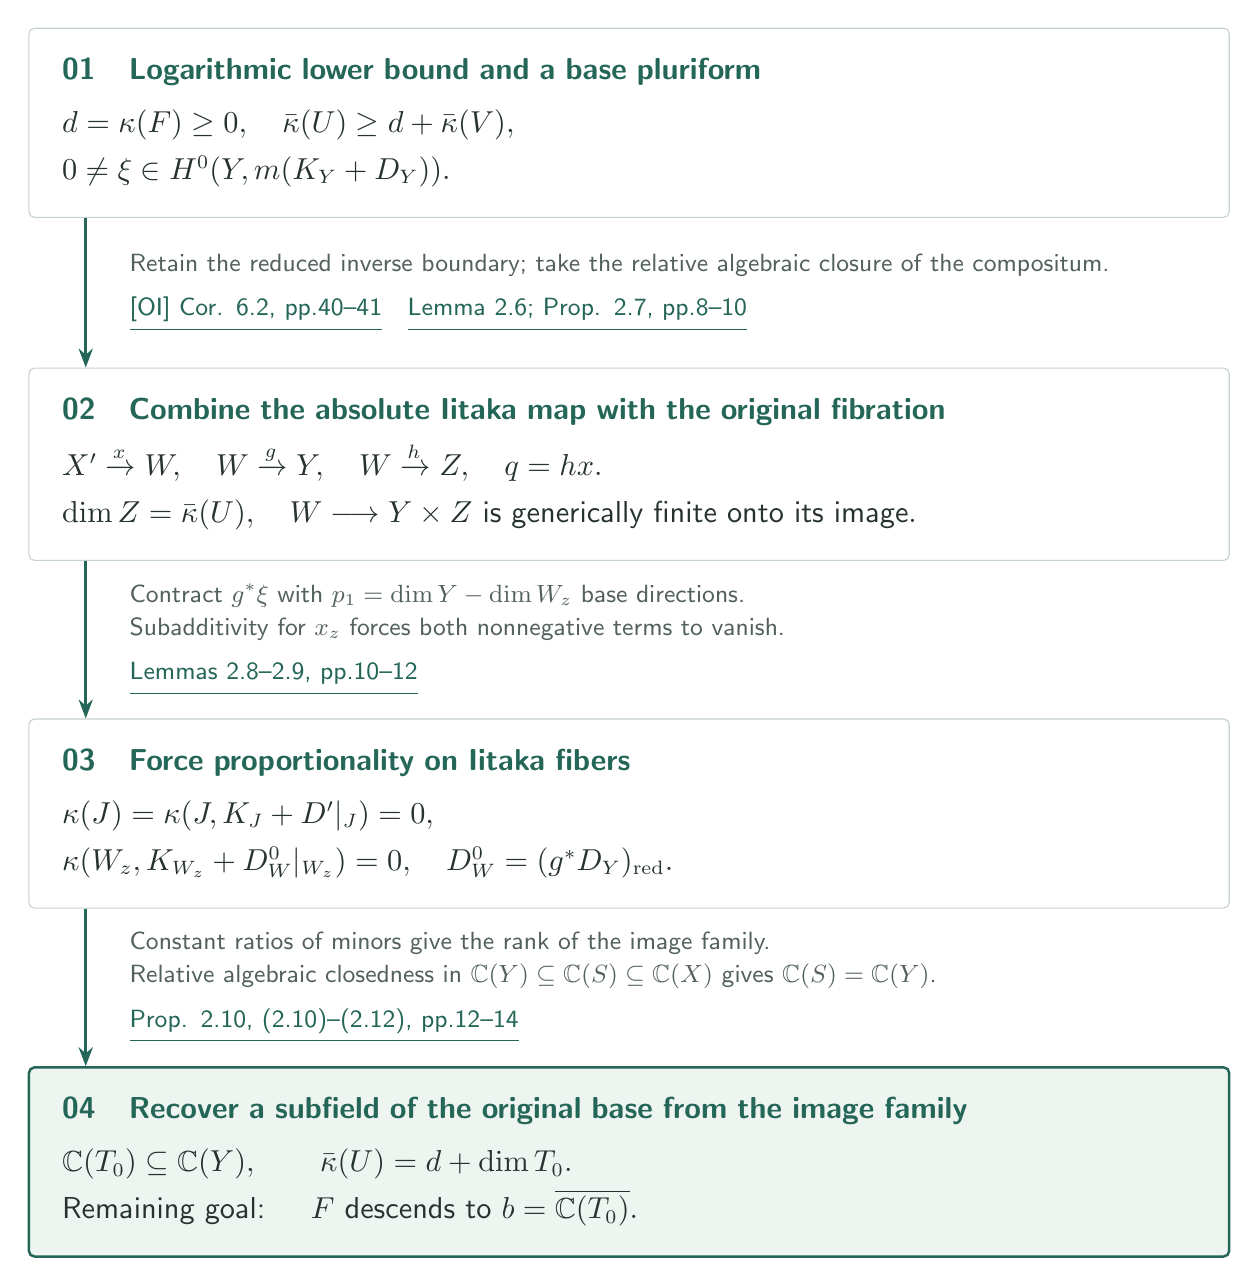
\begin{tikzpicture}
\node[card] (start) {\heading{01}{対数的下界と非零の底の形式}{Logarithmic lower bound and a base pluriform}
$d=\kappa(F)\ge0,\quad \bar\kappa(U)\ge d+\bar\kappa(V),$
\\[3pt]$0\ne\xi\in H^0(Y,m(K_Y+D_Y)).$};
\node[card,below=1.9cm of start] (combined) {\heading{02}{絶対飯高写像と元の射を合わせる}{Combine the absolute Iitaka map with the original fibration}
$X'\xrightarrow{x}W,\quad W\xrightarrow{g}Y,\quad W\xrightarrow{h}Z,\quad q=hx.$
\\[3pt]$\dim Z=\bar\kappa(U),\quad W\longrightarrow Y\times Z\ \Tx{\text{は像上generically finite}}{\text{is generically finite onto its image}}.$};
\flow{start}{combined}{\Tx{係数1の逆像境界を保つ。合成体の相対代数閉包で中間体を選ぶ。}{Retain the reduced inverse boundary; take the relative algebraic closure of the compositum.}\\[4pt]
\R{OI}{[OI] Cor. 6.2, pp.40--41}\quad\R{WV}{Lemma 2.6; Prop. 2.7, pp.8--10}}
\node[card,below=2cm of combined] (zero) {\heading{03}{飯高ファイバー上の切断を比例させる}{Force proportionality on Iitaka fibers}
$\kappa(J)=\kappa(J,K_J+D'|_J)=0,$\\[3pt]
$\kappa(W_z,K_{W_z}+D_W^0|_{W_z})=0,\quad D_W^0=(g^*D_Y)_{\rm red}.$};
\flow{combined}{zero}{\Tx{$g^*\xi$ を $p_1=\dim Y-\dim W_z$ 個の底方向で収縮する。\\$x_z$ への劣加法性で、非負の二項がともに0となる。}{Contract $g^*\xi$ with $p_1=\dim Y-\dim W_z$ base directions.\\Subadditivity for $x_z$ forces both nonnegative terms to vanish.}\\[4pt]
\R{WV}{Lemmas 2.8--2.9, pp.10--12}}
\node[result,below=2cm of zero] (field) {\heading{04}{像の族から、元の底の部分体を得る}{Recover a subfield of the original base from the image family}
$\C(T_0)\subseteq\C(Y),\qquad\bar\kappa(U)=d+\dim T_0.$\\[3pt]
$\Tx{\text{残る目標：}}{\text{Remaining goal: }}\quad F\ \Tx{\text{を }b=\overline{\C(T_0)}\text{ 上へ降下}}{\text{descends to }b=\overline{\C(T_0)}}.$};
\flow{zero}{field}{\Tx{小行列式の比の一定性から像の族の階数を得る。\\$\C(Y)\subseteq\C(S)\subseteq\C(X)$ と相対代数閉性が $\C(S)=\C(Y)$ を与える。}{Constant ratios of minors give the rank of the image family.\\Relative algebraic closedness in $\C(Y)\subseteq\C(S)\subseteq\C(X)$ gives $\C(S)=\C(Y)$.}\\[4pt]
\R{WV}{Prop. 2.10, (2.10)--(2.12), pp.12--14}}
\end{tikzpicture}

\end{document}
